
% Change dir here
\def\covmac{/Users/matiascovarrubias/Documents/universidad/NYU/Research/Repositories/marketsAI/marketsai/Documents/Figures}
\let\dir=\covmac
%\documentclass[compress]{beamer} % notesonly

\documentclass[serif,9pt]{beamer}

\usepackage{palatino}
\usepackage{beamerthemesplit}
\usepackage{epsfig}
\usepackage{mathpazo}
\usepackage{soul}
\usepackage{setspace}
\usepackage{hyperref}
\usepackage{graphicx}
\graphicspath{{Figures/}}
\usepackage{amsmath,amssymb}
\usepackage{spot}
\usepackage{tikz}
\usepackage{wasysym}
\usepackage{subcaption}
\newcommand{\pyobject}[1]{\fbox{\color{red}{\texttt{#1}}}}
\newcommand{\cmark}{\ding{51}}%
\usepackage[outdir=./]{epstopdf}
\newcommand{\rectangle}{\fboxsep0pt\fbox{\rule{1em}{0pt}\rule{0pt}{1ex}}}

\usepackage{float,graphicx}
\usepackage[justification=centering]{caption}
\usepackage{amsmath}
\usepackage{amssymb}
\usepackage{geometry}
\usepackage{color}
\newcommand\tsum{\textstyle\sum\nolimits}

\newcommand{\tlap}[1]{\raisebox{0pt}{#1}}
\newcommand{\myitem}[1]{\tlap{\rlap{\parbox[t]{\linewidth}{\item {\vspace{-2.2ex} \strut#1\strut}}}}}

\usetheme{CambridgeUS}
\usecolortheme{dolphin}

\newenvironment{myquote}{\list{} {\leftmargin=0.0in\rightmargin=0.3in \scriptsize \itshape }{}\item[]}{\endlist}

\newtheorem{prop}{Proposition}
\newtheorem{proposition}[theorem]{Proposition}

\newcommand{\ra}{$\rightarrow \hspace{0.1cm}$}
\newcommand{\Ra}{$\Rightarrow \hspace{0.1cm}$}
\newcommand{\Ua}{$\Uparrow \hspace{0.1cm}$}
\newcommand{\Da}{$\Downarrow \hspace{0.1cm}$}

\newcommand{\be}{\begin{equation}}
	\newcommand{\ee}{\end{equation}}
\newcommand{\bes}{\begin{equation*}}
	\newcommand{\ees}{\end{equation*}}
\newcommand{\bi}{\begin{itemize}}
	\newcommand{\ei}{\end{itemize}}
\newcommand{\ms}{\medskip}
\newcommand{\bs}{\bigskip}
\newcommand{\sms}{\smallskip}

\newcommand{\mhat}{\hat{\mu}}
\newcommand{\hmu}{\hat{\mu}}
\newcommand{\ahat}{\hat{a}}
\newcommand{\sa}{\sigma_a}
\newcommand{\si}{\sigma_i}
\newcommand{\sx}{\sigma_x}
\newcommand{\ha}{\hat{a}}
\newcommand{\shata}{\hat{\sigma}_a}
\newcommand{\hi}{\hat{s}_i}
\newcommand{\shati}{\hat{\sigma}_i}
\newcommand{\shat}{\hat{\sigma}}
\newcommand{\Shat}{\hat{\Sigma}}
\newcommand{\sna}{\sigma_{\eta a}}
\newcommand{\sno}{\sigma_{\eta 1}}
\newcommand{\snt}{\sigma_{\eta 2}}
\newcommand{\ex}{\bar{x}}
\newcommand{\epsi}{\varepsilon}
\newcommand{\p}[1]{\left( #1 \right)}
\newcommand{\h}{\mathcal{H}}
\newcommand{\M}{\mathcal{M}}
\newcommand{\E}{\mathbb{E}}
\newcommand{\V}{\mathcal{V}}
\newcommand{\La}{\mathcal{L}}
\newcommand{\W}{\mathcal{W}}
\newcommand{\T}{\mathbb{T}}
\newcommand{\dom}{\mathcal{D}}
\newcommand{\pc}{\perp_C}
\newcommand{\vecspan}{\operatorname{span}}
\newcommand{\interior}{\operatorname{int}}
\newcommand{\lcm}{\operatorname{lcm}}
\newcommand{\tr}{\operatorname{tr}}
\newcommand{\divides}{|}
\newcommand{\claim}{Claim: }
\newcommand{\tmu}{\tilde{\mu}}
\newcommand{\wt}[1]{\widetilde{#1}}
\newcommand{\wb}[1]{\overline{#1}}
\newcommand{\wh}[1]{\widehat{#1}}
\newcommand{\pare}[1]{\left( #1 \right)}

\newcommand\smallfont{ \usefont{T1}{ptm}{m}{n}\fontsize{9pt}{9pt}\selectfont\DB}
\newcommand\verysmallfont{\usefont{T1}{ptm}{m}{n}\fontsize{8pt}{8pt}\selectfont}%
\renewcommand{\cite}{\citeasnoun}
\renewcommand<>{\sout}[1]{\alt#2{\beameroriginal{\sout}{#1}}{#1}}
\def\DPbar{\overline{DP}}


\newtheorem{result}[theorem]{Result}

\definecolor{green}{RGB}{0 200 0}
\definecolor{purple}{RGB}{138 	43 	226 	}
\definecolor{limegreen}{RGB}{50 205 50}

\usepackage{tikz}
\usetikzlibrary{shapes}
\usetikzlibrary{fadings}

\tikzfading[name=spotfade2,
inner color=transparent!100,
outer color=transparent!20]
\definecolor{colorspot}{RGB}{    255  255 0}



\tikzfading[name=spotfade,
inner color=transparent!100,
outer color=transparent!80]

\setspotlightstyle{ball color=cyan,fill=cyan, path fading=spotfade, draw=cyan, thick }

\title{Deep Reinforcement Learning in Macroeconomic Models}
\author[Covarrubias]
{Matias Covarrubias}
\institute[NYU]{NYU}

\date[]{}

\setbeamertemplate{navigation symbols}{}

\begin{document}
\begin{frame}
  \titlepage
\end{frame}

\section{Introduction}
%%% SLIDE 1 %%%
\begin{frame}
\frametitle{This paper}
\begin{itemize}

\item Two questions: \medskip

\begin{itemize}
	\item Can artificial intelligent (AI) algorithms learn optimal intertemporal behavior without knowing any mathematical details of the economy beforehand? \medskip
	\item How should we specify economies and markets so as to make them easy to learn? 
\end{itemize}

\item I apply Deep Reinforcement Learning (Deep RL)  to macroeconomic problems. \medskip

\item  In the context of an investment under uncertainty model with heterogeneous agents, I show that Deep RL agents can learn the rational expectations solution and I suggest design choices that aid such learning. \medskip

\item Then, by manipulating our baseline framework I highlight three topics in which this technology can be useful:   \medskip
\begin{itemize}
	\item high dimensional problems. \ms
	\item incomplete information problems. \ms
	\item equilibrium selection in models with multiple equilibrium. \ms
\end{itemize},

\end{itemize}
\end{frame}

\begin{frame}
\frametitle{An overview of Reinforcement Learning}

\begin{itemize}
	\item  RL is a class of algorithms that adapt dynamic programming techniques to the problem of online learning, that is, to learn how to control a system by interacting and experimenting with it. \medskip
	
	\item They do not use any mathematical knowledge of  the system they are controlling, other than the allowed actions and states. \medskip
	
	\begin{itemize}
		\item They feed actions to the system and observe the reward they get that period and how the state evolves.  \medskip
		\item After many transitions, if  successful, they are able to estimate the consequences of their actions accurately and thus make optimal decisions. \medskip
	\end{itemize}

	\item  Deep RL adds neural nets as function approximators. It has shown state of the art performance in many tasks such as: \medskip
	
	\begin{itemize}
		\item Games, including complex multi-agent games. (cite) \medskip
		\item Robotics. ( cite) \medskip
		\item Autonomous driving. (cite) \medskip
		\item Operations research. (cite) \medskip
	\end{itemize}
\end{itemize}
\end{frame}

\begin{frame}
\frametitle{Online Learning}
\begin{figure}
	\centering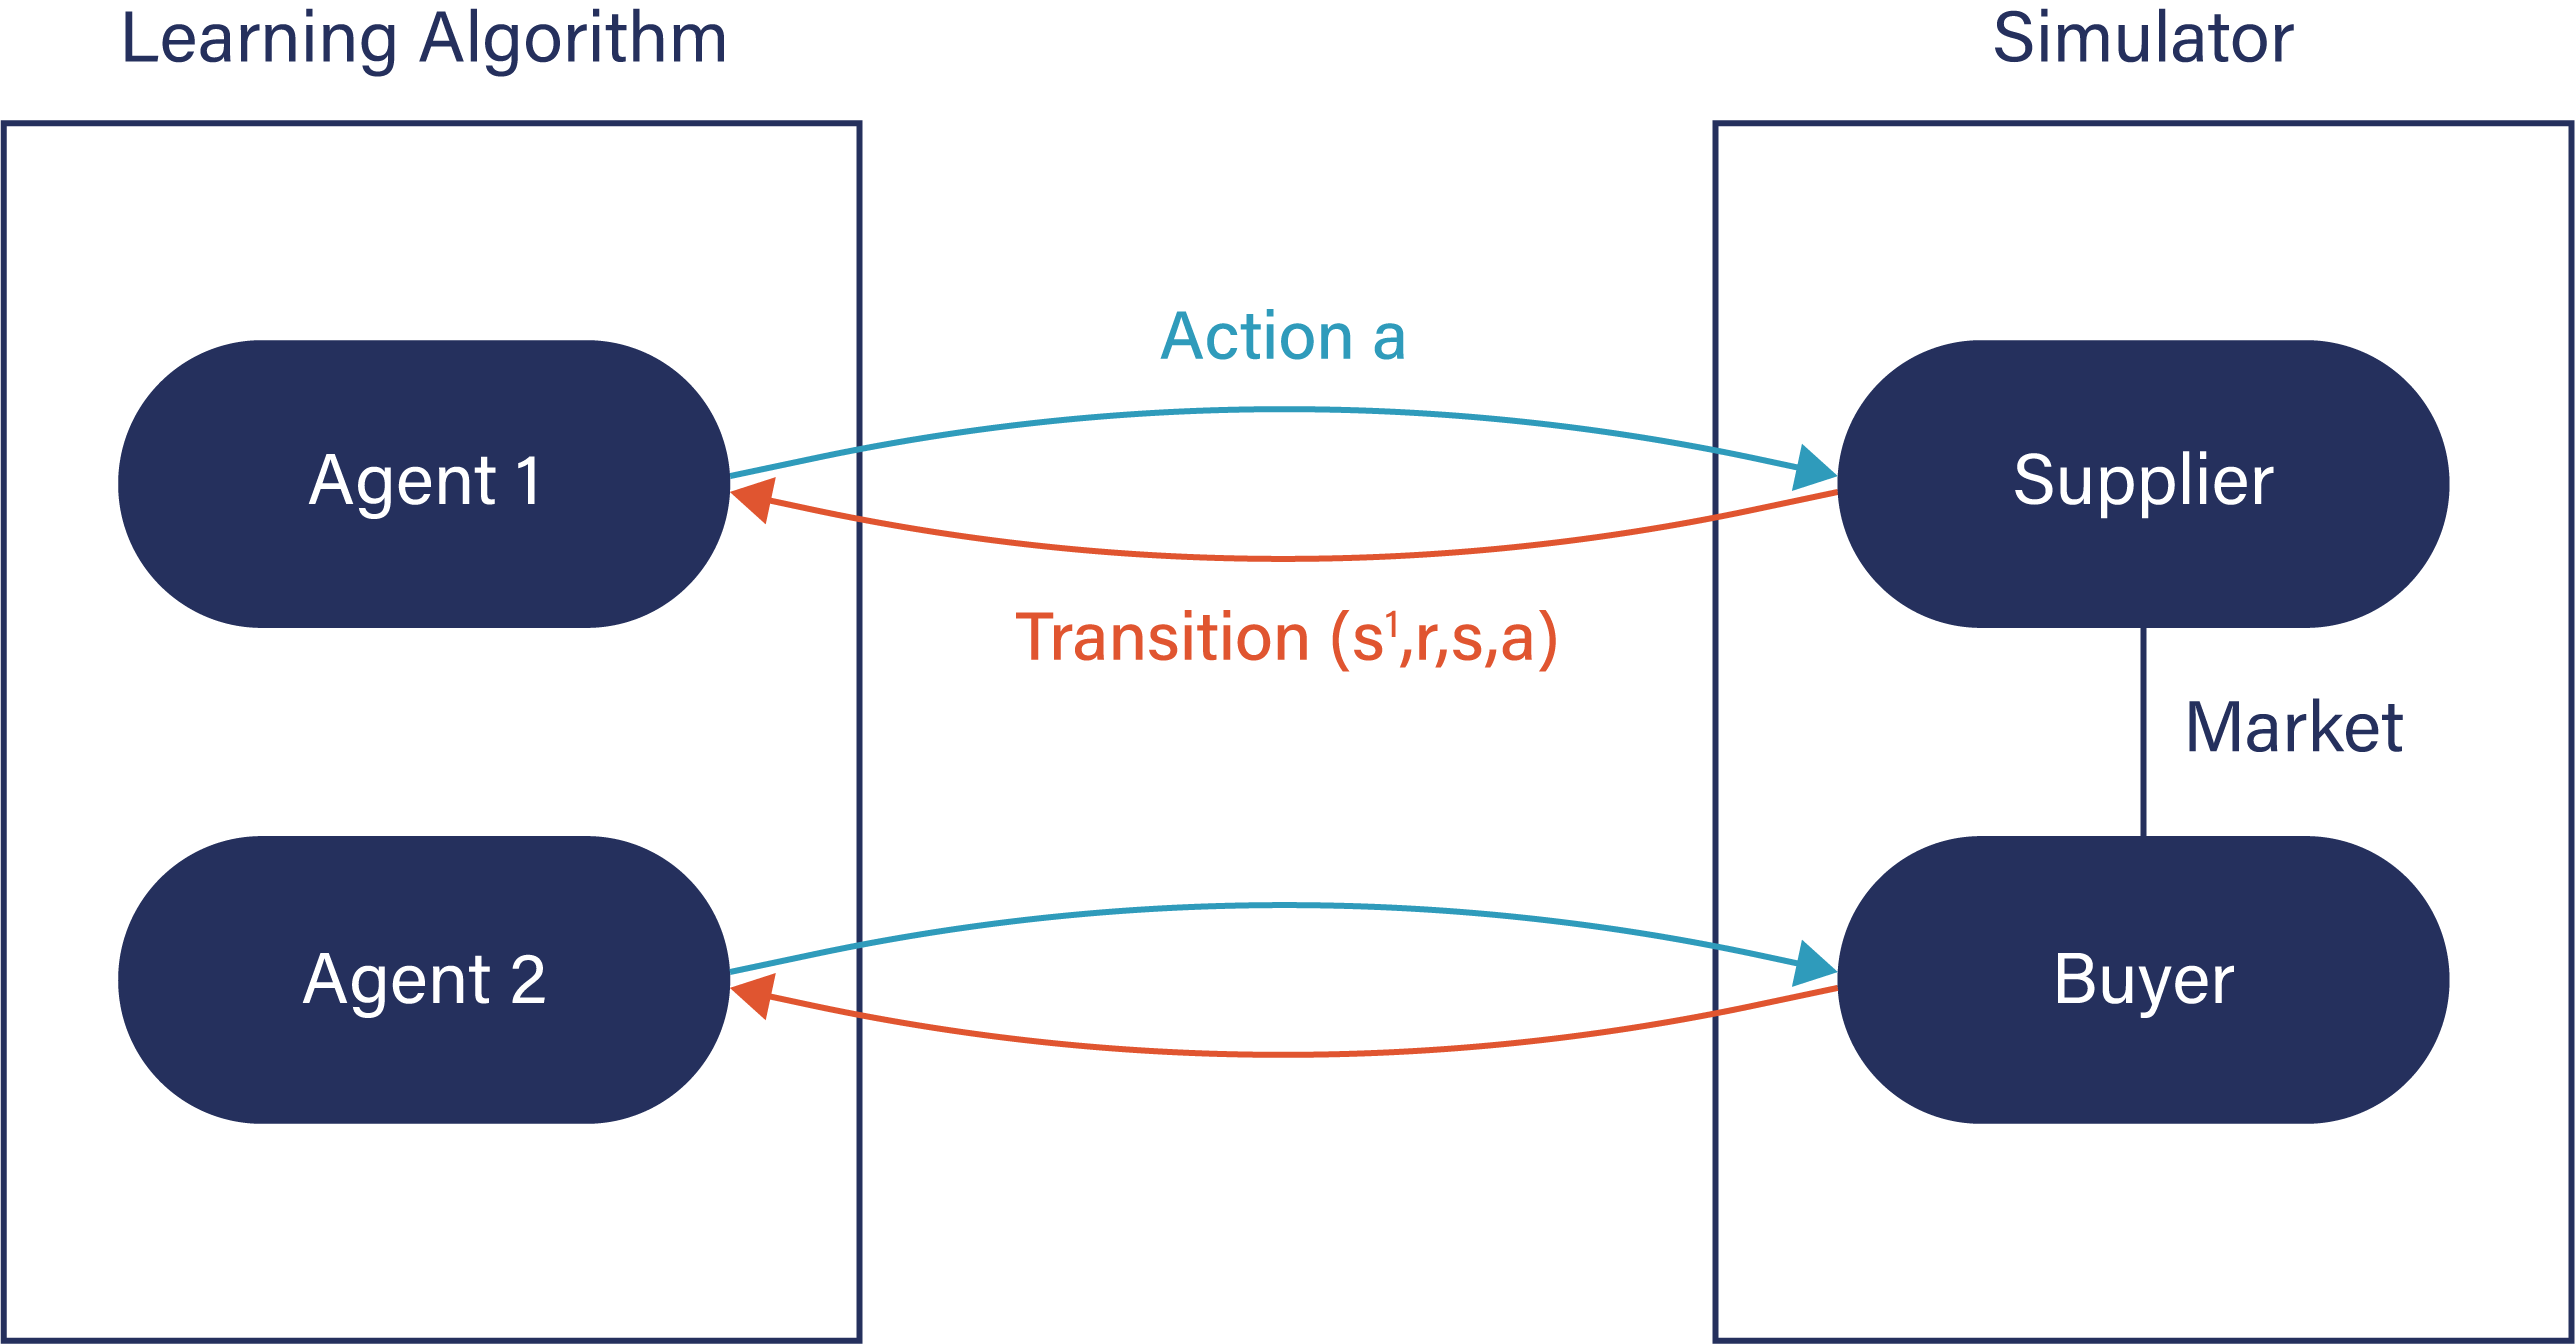
\includegraphics[scale=0.2]{\dir/Online-learning.png}
	\caption{Online learning workflow}
\end{figure}
\end{frame}

\begin{frame}
\frametitle{Deep RL in economics?}

\begin{itemize}
	
	\item Traditional challenges of Deep RL and why economics may be particularly well suited for this technology.\medskip

\begin{itemize}
	\item Rewards engineering is usually the main bottleneck. In economics, rewards are well specified in every period. \medskip
	
	\item RL algorithms usually require millions of transitions in order to learn.  In economics, sampling a transition is usually very fast. \medskip
	
	\item Algorithms may get stuck in local optima. In many problems, we  have nice regularity properties. \medskip
\end{itemize}


\item  But, economic problems present their own challenges. \medskip

\begin{itemize}
	\item Markets are a multi-agent problem. Challenge: agents learn and explore while other agents learn and explore $\to$ environment is not stationary. \medskip
	
	\item In economics, rigorous insights often rely on exact solutions. That is, we are trying to solve very precise control problems.  \medskip
\end{itemize}	
\end{itemize}

\end{frame}

\section{Framework}
%%% SLIDE 2 %%%
\begin{frame}
\frametitle{An economy in an RL framework}

We formalize an economy as a a Partially Observed Markov Game. In each period:\medskip

\begin{itemize}
	\item $n$ agents indexed by $i$ choose an action $a_i \in \mathcal{A}_i$, after observing a state $s_i \in \mathcal{S}_i $. \medskip
	
	\item Let $\mathcal{S}$ be set of states, that is, the collection of all possible states $S_i$. \ms 
	
	\item The initial states are determined by a distribution $\rho:\mathcal{S} \mapsto [0,1]$.\medskip
	
	\item To choose actions, each agent $i$ uses a stochastic policy $\pi_{\theta_i}: \mathcal{S}_i \times \mathcal{A}_i \mapsto [0,1]$. \ms
	
	\item The combined actions produces the next state according to the state transition function $p:\mathcal{S} \times \mathcal{A}_i \times ... \times \mathcal{A}_N \mapsto \mathcal{S}$. \medskip
	
	\item Each agent $i$ observes its reward as a function of the state and agent's action $r_i:\mathcal{S} \times  \mathcal{A}_i \times ... \times \mathcal{A}_N \mapsto \mathcal{R}$, and receives a private observation  $s'_i: \mathcal{S} \mapsto \mathcal{S}_i$.  \medskip
	
	
\end{itemize}
\end{frame}



\begin{frame}
\frametitle{Overview of baseline framework}

\begin{itemize}

	\item My criteria for choosing a baseline framework are the following: \medskip

\begin{itemize}
	\item Simple economics, challenging solution: the problem should be easy to explain and with clear economics. \medskip
	
	\item Dynamics at the forefront: the key trade-offs of the model should be intertemporal. \medskip
	
	\item Meaningful scalability: the problem needs to have a clear path to scalability. It cannot have aggregation properties. \medskip
\end{itemize}

\item  I present a version of the stochastic growth model in which we focus on the purchase market for capital goods and introduce heterogenous agents.  \medskip

\item $N^h$ households produce the final good and  choose how much consume vs invest.\medskip

\item The final good is produced using bundle of $N^c$ capital goods.    \medskip

\item  The cost of producing new capital goods is quadratic in \textbf{aggregate} investment.  \medskip

\item  We will consider both a  market's formulation and a planner's formulation of the problem.


\end{itemize}

\end{frame}

\begin{frame}
\frametitle{4 experiments}


\begin{enumerate}
	\item Experiment 1: Planner formulation of stochastic growth model with many households and aggregate convex cost of adjustment.\ms
	
	
	\begin{itemize}
		\item Single-agent $\to$ control problem is exactly the same as the one we solve in economics.  \ms
		
		\item We learn: \ms 
		\begin{enumerate}
			\item Deep RL agent learn optimal solution consistent with rational expectations.  \ms
			\item It can quickly solve high dimensional problems. \ms
		\end{enumerate}
		
	\end{itemize}
	
	\item Experiment 2: Market formulation of the problem with a competitive supply. \ms
	
	\begin{itemize}
		
		\item Multi-agent problem: can be formalized as Partially Observed Markov Games $\to$ few theoretical guarantees. \ms
		
		\item Challenge: non-stationarity. Agents learn while others are learning (and experimenting) as well. \ms
		
		\item We learn:
		
		\begin{enumerate}
			\item Order arises from chaos and agents find a solution. \ms
			\item Deep RL agents behave strategically and they consider their effect on prices. \ms
		\end{enumerate}
	\end{itemize}
	
	
	
\end{enumerate}

\end{frame}

\begin{frame}
\frametitle{4 experiments (continued)}


\begin{enumerate}

\item Experiment 3: Incomplete information.  \ms

\begin{itemize}
	
	\item Half of the households have full information, half observes only own state plus aggregate statistics of other's state. \ms
	
	\item The point of this experiment is to illustrate how easy is to modify the informational structure of the economy. \ms
	
	\item We can calculate the gain in expected utility of the additional information. \ms
	
\end{itemize}
\item Experiment 4: Deep RL agents in both supply and demand  \ms

\begin{itemize}
	
	\item Challenging because we cannot use walrasian auctioneers to guarantee market clearing. \ms
	
	\item I explore alternative formulations of the market game and check whether increasing the number of sellers and buyers get the solution closer to competitive solution. \ms
	
	
\end{itemize}

\end{enumerate}

\end{frame}


%%% SLIDE 2 %%%
\begin{frame}
\frametitle{To start: Planner formulation, 1 Household, 1 capital good}
\begin{itemize}
	\item A representative household chooses how much to consume and how much to invest in order to maximize $\sum_{t=0}^{\infty} \beta^t u(c_t)$.\medskip
	
	\item The final good is produced using capital $K$ according to the production function $Y=Z K^{\alpha}$. The agent needs to decide how much of that product to consume and how much to use for production of new capital goods. \medskip
	
	\item \textbf{Adjustment costs:} In order to produce $I_t$ new capital goods the representative agent needs to sacrifice $\frac{\phi}{2} I^2_t$ final goods.  \medskip
	
	\item We express the problem in terms of choosing the saving rate $s$ such that consumption is $C_t=(1-s_t)Y_t$ and investment is defined by the equation $\frac{2}{\phi} I_t^2 = s_t Y_t$. Thus: \medskip
	
	$$I_t = \sqrt{\frac{2}{\phi} s_t Y_t}$$
\end{itemize}

\end{frame}

\begin{frame}
\frametitle{Planner, 1HH, 1 capital: recursive formulation}

\begin{itemize}
	\item The recursive formulation of the problem is: \medskip
	
	
	\begin{align*}
	V_t\left(K_t, Z_t\right) = &\max_{s_t,K_{t+1}} U(C_t) + \beta \E_t V_{t+1}(K_{t+1}, Z_{t+1}) \qquad \text{s.t.}\\
	&\qquad
	C_t = Y_t(1-s_t)\\
	&\qquad
	Y_t = Z_t K_t^\alpha\\
	&\qquad
	K_{t+1} \leq (1-\delta) K_t + \sqrt{\frac{2}{\phi} s_t Y_t}
	\end{align*}
	
	where $Z_t$ follows a markov chain with transition probability $\mathcal{P}$.

\end{itemize}

\end{frame}

\begin{frame}
\frametitle{ Planner, $N^h$ HHs, 1 capital }
\begin{itemize}
\item A key part of the problem with many households is that the covex adjustment cost are over the total amount of produced capital. \medskip

 \item For the planner formulation, we assume that all the resources that are committed by households are  employed in production, and then total production is distributed among households according to their contribution. Total production is defined implicitly by:

$$\sum_{i=1}^{N^h} s_{i,t} Y_{i,t} = \frac{\phi}{2} I^2$$

where $i$ indexes a household. Solving for $I_{t}$ we get:

$$I_{t} =  \sqrt{\frac{2}{\phi} \sum_{i=1}^{N^h} s_{i,t} Y_{i,t}}$$

We can then distribute it among households according to

$$I_{i,t} = \frac{s_{i,t}Y_{i,t}}{ \sum_{i=1}^{N^h} s_{i,t} Y_{i,t}}  I_{t} =   \frac{s_{i,t}Y_{i,t}}{\sqrt{\frac{\phi}{2} \sum_{i=1}^{N^h} s_{i,t} Y_{i,t}}}$$
\end{itemize}

\end{frame}

\begin{frame}
\frametitle{ Planner, $N^h$ HHs, 1 capital: recursive formulation}

\begin{itemize}
	\item The recursive formulation of the problem is:

\begin{align*}
V\left(\{K_{i,t}, Z^{id}_{i,t} \}_{i}, Z^{agg}_t\right) = &\max_{\{s_{i,t},K_{i,t+1}\}_{i}} \sum_{i=1}^{N^h} U(C_{i,t}) + \beta \E_t V((\{K_{i,t+1}, Z^{id}_{i,t+1} \}_{i}, Z^{agg}_{t+1}) \qquad \text{s.t.}\\
&\qquad
C_{i,t} = (1- s_{i,t})Y_{i,t} \quad \text{for } i \in [1,...,N^h]\\
&\qquad
Y_{i,t}=Z^{agg}_{t} Z^{id}_{i,t}  K_{i,t}^{\alpha}  \quad \text{for } i \in [1,...,N^h]\\
&\qquad
K_{i,t+1} \leq (1-\delta) K_{i,t} + \frac{s_{i,t}Y_{i,t}}{\sqrt{\frac{\phi}{2} \sum_{i=1}^{N^h} s_{i,t} Y_{i,t}}} \quad \text{for } i \in [1,...,N^h]
\end{align*}
	
	where $Z^{agg}_t$ and  ${Z^{id}_{i,t}}_i$ follow markov chains with transition probability $\mathcal{P}^{agg}$ and $\mathcal{P}^{ind}$.
	
\end{itemize}

\end{frame}

\begin{frame}
\frametitle{Market, $N^h$ HHs, 1 capital: household problem}

\begin{itemize}
	\item  First, we assume that there is a market for investment goods and we introduce capital good firms that pay the adjustment cost and sell the investment good at price $p^k_{t}$. Thus, from the point of view of the household, investment is $I^h_{i,t} = s_{i,t}/p^k_{t}$.   \medskip
	
	\item The recursive formulation of the problem for household $i$ is:
	
	
	\begin{align*}
	V_i \left(\{K_{i,t}, Z^{id}_{i,t} \}_{i}, Z^{agg}_t \right) = &\max_{\{s_{i,t},K_{i,t+1}\}_{j}}  U(C_{i,t}) + \beta \E_t V_i((\{K_{i,t+1}, Z^{id}_{i,t+1} \}_{i}, Z^{agg}_{t+1}) \qquad \text{s.t.}\\
	&\qquad
	C_{i,t} = (1- s_{i,t})Y_{i,t} \\
	&\qquad
	Y_{i,t}=Z^{agg}_{t} Z^{id}_{i,t}  K_{i,t}^{\alpha}\\
	&\qquad
	K_{i,t+1} \leq (1-\delta) K_{i,t} + \frac{s_{i,t} Y_{i,t}}{p^k_{t}}  
	\end{align*}
	
\end{itemize}

\end{frame}

\begin{frame}
\frametitle{Market, $N^h$ HHs, 1 capital: capital good firm}

\begin{itemize}
	
	\item At first, we will assume that the capital producer is price taker: \medskip
	
	\begin{itemize}
		\item It maximizes 	$$\pi^c_{t}=p^k_{t} I^c_{t}-\frac{\phi}{2} \left(I^c_{t}\right)^2 $$. \medskip
		
		\item Price is then determined by 	 $$p^k_{t} = \phi I^c_{t}$$ \medskip
		
	\end{itemize}

	\item Then, in order to study strategic behavior in environments where both buyers and sellers are Deep RL agents,  we will allow a deep RL agent to fix the mark-up over price. 
	
\end{itemize}
\end{frame}

\begin{frame}
\frametitle{Market, $N^h$ HHs, $N^c$ capital goods.}

\begin{itemize}
	\item Now we have $N^c$ capital goods indexed by $j$.   \medskip
	
	\item The recursive formulation of the problem for household $i$ is:
	
	\begin{align*}
V_i \left(\{K_{i,j,t}\}_{i,j}\right) = &\max_{\{s_{i,j,t},K_{i,j,t+1}\}_{j}}  U(C_{i,t}) + \beta \E_t V_i(\{K_{i,j,t+1}\}_{i,j}) \qquad \text{s.t.}\\
&\qquad
C_{i,t} = (1-\sum_{j=1}^{N^c} s_{i,j,t})Y_{i,t} \\
&\qquad
Y_{i,t}=Z^h_{i,t} \Pi_{j=1}^{N^c} K_{i,j,t}^{\alpha/N^c}\\
&\qquad
K_{i,j,t+1} \leq (1-\delta) K_{i,j,t} + \frac{s_{i,j,t} Y_{i,t}}{p^k_{j,t}}  \quad \text{for } j \in [1,...,N^c] 
\end{align*}

\item The supply is give by the equation $p^k_{j,t} = \phi I^c_{j,t}$ where 

\end{itemize}

\end{frame}

\section{Learning Algorithms}

%%% SLIDE 11 %%%

\begin{frame}
\frametitle{Reinforcement Learning Algorithm}

\begin{itemize}
	\item We start from simplest single agent algorithm. The problem is: \ms
	$$\underset{a \in A}{\max} \sum_{t=s}^{\infty} \gamma^{s-t} E_t[r_{t+s}]$$
	
	\item Two value functions:\ms
	\begin{enumerate}
		\item state-value function: $V(s)=\max_{a\in A} \{E[r|s,a] + \gamma E[V(s')|s,a] \}$ \medskip
		\item action-value function: $Q(s,a)=E(r|s,a)+\gamma E[\max_{a'\in A} Q(s',a')|s,a]$ \medskip
	\end{enumerate}
	\item Q-Learning: \ms
	\begin{itemize}
		\item Initialize $Q_0(s,a)$. Loop until converge: \ms
		\begin{itemize}
			\item agent chooses $a= \text{arg} \max Q(s,a)$  and observes $\{r, s'  ,s, a\}$. \ms
			\item Old Q: $Q(s,a)$. \ms
			\item  Target Q: $r_t+\gamma \max_{a' \in A} Q(s',a')$. \ms
			\item New Q: $$Q'(s,a)=(1-\alpha) Q(s,a) +\alpha [r+\gamma \max_{a' \in A} Q(s',a')]$$ \ms
		\end{itemize}
	\end{itemize}
\end{itemize}

\end{frame}

%%% SLIDE 3 %%%
\begin{frame}
\frametitle{Getting deeper: Deep RL}

\begin{itemize}
\item Deep Q-learning consists in approximating the Q function with a neural net: $\hat{Q}(s,a) \equiv  \mathcal{N}_\rho \sim Q(s,a)$.\ms
\item The parameters $\rho$ are estimated in order to minimize \ms
$$\mathcal{L}(\rho)=\E \left[ \left(\hat{Q}(s,a)-(r_t+\gamma \max_{a' \in A} \hat{Q}(s',a')) \right)^2 \right] $$

in observed transitions $\{r, s'  ,s, a\}$ .\ms

\item A common example of a NN is a composite function made of nested linear functions:  \ms

$$\mathcal{N}_\rho (x)=\sigma_K(W_K ... \sigma_2(W_2 \sigma_1(W_1x+b_1)+b_2)...+b_K)$$

where $x$ is the input (in our case the transitions $\{r, s'  ,s, a\}$), $W_i \in \mathbb{R}^{m_{i+1}\times m_i}$ are the weights, $b_i \in \mathbb{R}^{m_i+1}$ are the biases, and $\sigma()$ are activation functions.
\end{itemize}

\end{frame}

\begin{frame}
\frametitle{Convergence results in RL}


\begin{itemize}
\item  Tsitsiklis (1994) If state space and action space are discrete, Q-learning converges globally if: \ms
\begin{itemize}
\item All state-action pairs are visited infinitely often. \ms
\item Conditions on learning rate $\alpha$. The sum $\sum_{t=0}^{\infty} \alpha_t^2$ is finite and $\sum_{t=0}^{\infty} \alpha_t$ is infinite. \ms
\end{itemize}

\item Tsitsikli and Van Roy (1997) prove convergences in the case of linear function approximators and Maei et al (2009) prove convergence with smooth non-linear approximators (e.g., neural nets). \ms

\item For multi-agent, convergence is hard to prove. Muller et al (2019) show convergence in a large class of games to a solution concept they called $\alpha$-rank.
\end{itemize}


\end{frame}



\begin{frame}
\frametitle{Taxonomy of State of the Art Algorithms}

There are three objects that the agents can learn:


\begin{enumerate}
\item q function $Q(s,a)$ \ms
\begin{itemize}
\item \textbf{Q-based methods} use NNs to represent $Q(s,a)$.  \ms
\item off-policy method: the NN can learn from steps taken by any policy.  \ms
\item Model-free method.  \ms
\end{itemize}

\item policy function $\pi(s,a)$  \ms
\begin{itemize}
\item \textbf{Policy-gradient methods} use NN to represent $\pi(s,a)$.  \ms
\item on-policy method. the NN only learns from steps taken from optimal policy.  \ms
\item Model-free. More stable than $Q$ but less sample efficient.  \ms
\end{itemize}

\item Model $p(r,s'|s,a)$  \ms
\begin{itemize}
\item \textbf{Model-based methods} uses different methods to represent $p(r,s'|s,a)$.  \ms
\item In recent stage of development compared to other methods.  \ms
\end{itemize}
\end{enumerate}

\end{frame}


\begin{frame}
\frametitle{In practice: How to create environments and agents}

An environment consists of a \textbf{reset} and a \textbf{step} function. \ms

An agent consist of a \textbf{choose\_action} and a \textbf{learn} function. Loop: \ms

\begin{itemize}
	\item \pyobject{initial\_state=env.reset()}
	\begin{itemize}
		\item The reset function gives you the initial state.\ms
	\end{itemize}
	
	\item \pyobject{action = agent.choose\_action(state)}
	\begin{itemize}
		\item takes the state as input and choose the optimal action. \ms 
	\end{itemize}
	
	\item \pyobject{next\_state, rewards = env.step(actions)} 
	\begin{itemize}
		\item Takes as input the actions of all the players and outputs the rewards for all the agents and the next state. \ms
	\end{itemize}
	
	\item \pyobject{agent.learn(r,s',s,a)} 
	\begin{itemize}
		\item  Takes as input the transition info $\{r,s',s,a\}$ and updates the internal estimates (e.g., policy functions).\ms
	\end{itemize}
	
	
\end{itemize}

\end{frame}

\section{Results}

\begin{frame}
\frametitle{Experiment 1: Results}

 We start with the plannner's problem. Exercises: \ms

	\begin{itemize}
		\item We vary the number of households ($N^h \in \{1,2,5,10,100\}$) to evaluate scalability. \medskip
		
		\item Two ways to formulate planner  solutions 
		\begin{enumerate}
			\item Single-agent maps global state $S$ to $N^h$ actions.  \ms
			\begin{itemize}
				\item Pro: Environment need only to expose the global state.  \ms
				\item Con:  Does not impose simmetry, so it needs to calculate probabilities of taking each of  $N^h$ actions $\to$ slower for normal sized states. \ms
			\end{itemize}
			\item Centralized learner learns policy that maps individual states $S_i$ to one action. All households receive same aggregate reward.  \ms
			\begin{itemize}
				\item Pro: imposes symmetry so it learns fast. Also, implementation is a couple of lines of code of difference with decentralized solution. \ms
				\item Con: The environment exposes a dictionary giving a reorder version of the global state for each houshold  $\to$ slow transitions due to information overhead. \ms
			\end{itemize}
		\end{enumerate} 
	\end{itemize}


\end{frame}

\begin{frame}
\frametitle{Planner, 1 household. Exact solution vs Learned policy}

\begin{itemize}
	\item We can compare the discounted utility on a simulated time window of a 1000 periods. 
	\begin{figure}
		\centering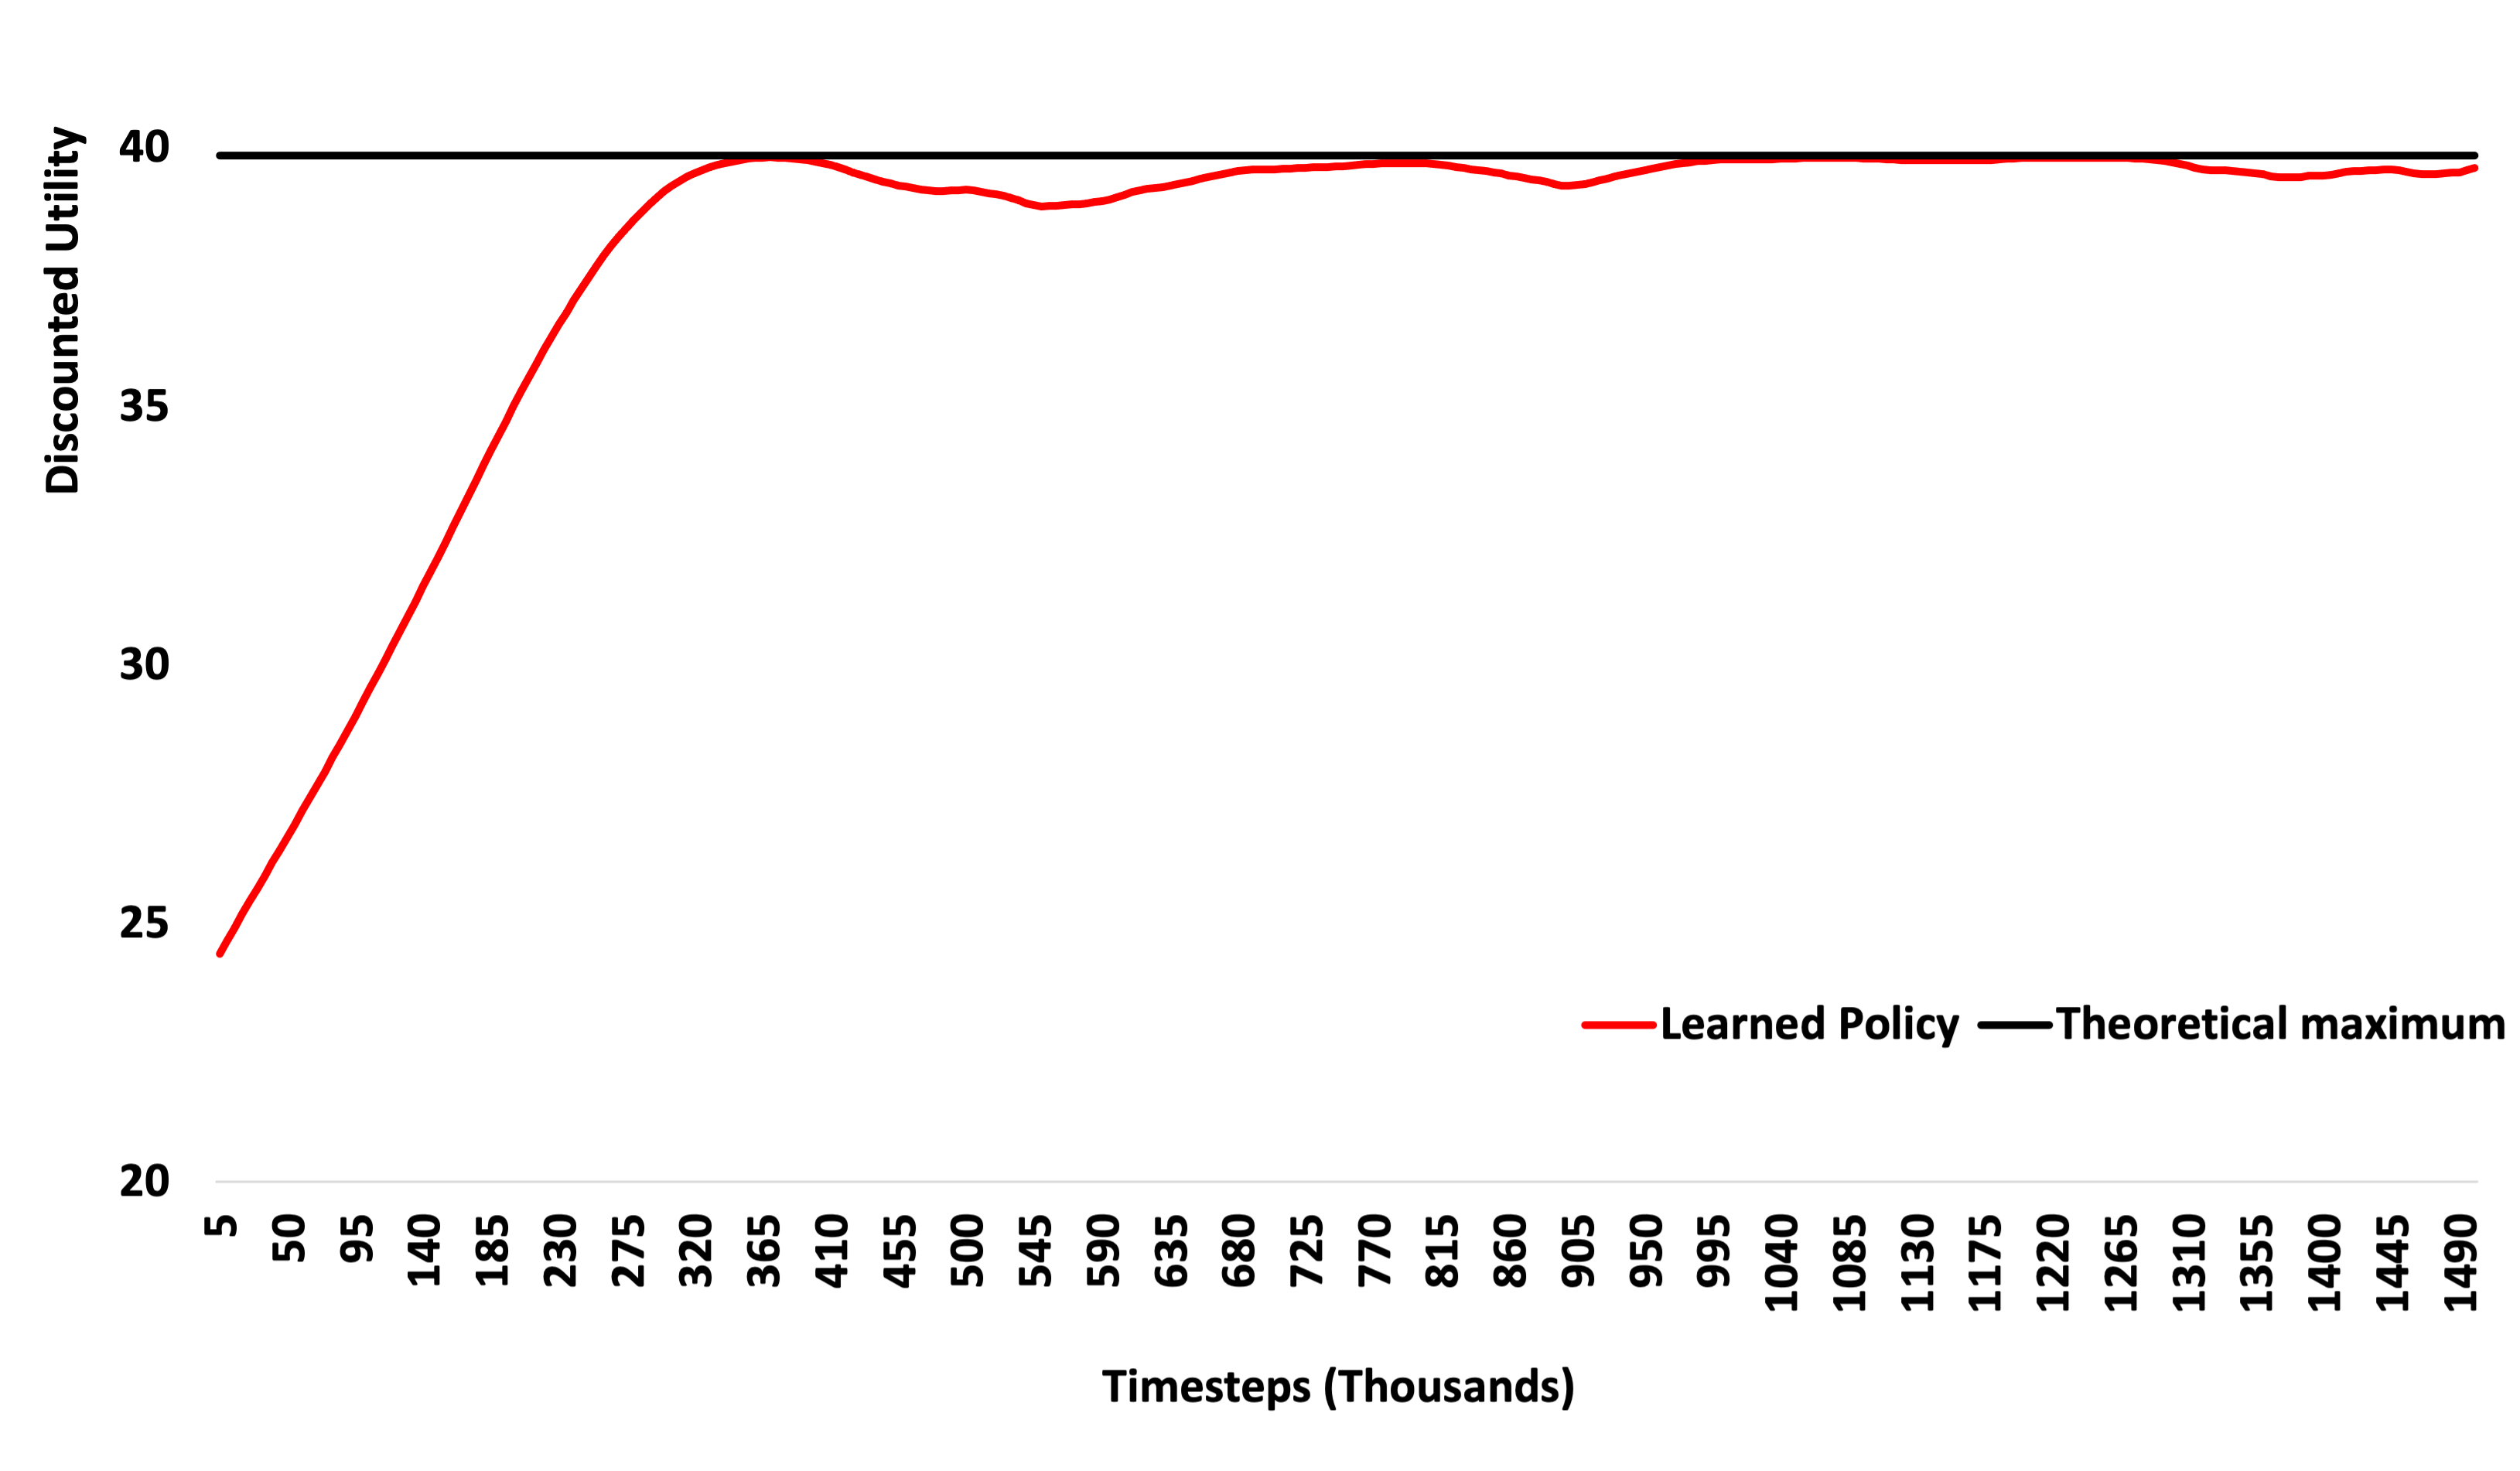
\includegraphics[scale=0.3]{\dir/econ_vs_RL_learning.png}
	\end{figure}
	
	\item The RL policy has a discounted utility that is 99.991\% of the discounted utility under the optimal policy. 
\end{itemize}
\end{frame}

\begin{frame}
\frametitle{Planner, 1 household. Simulating the exact solution vs Learned policy}

\begin{itemize}
	\item We simulate a series of shocks and compare the optimal poly calculated through policy iteration vs the policy learned trough Deep RL. 
\begin{figure}
	\centering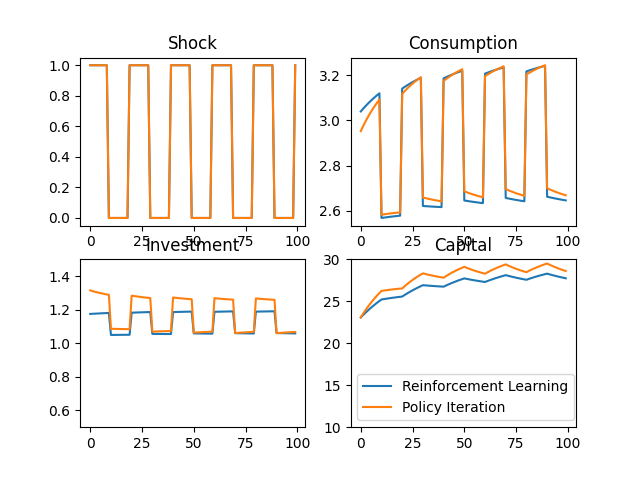
\includegraphics[scale=0.5]{\dir/capital_planner_IRecon_Aug3_1hh.png}
\end{figure}

	\item We still observe differences differences in time series.
\end{itemize}
\end{frame}

\begin{frame}
\frametitle{Planner, Learning charts by number of households}

\begin{itemize}

\item We compare the number of transitions it takes to reach peak performance according to number of households.

\begin{figure}
	\centering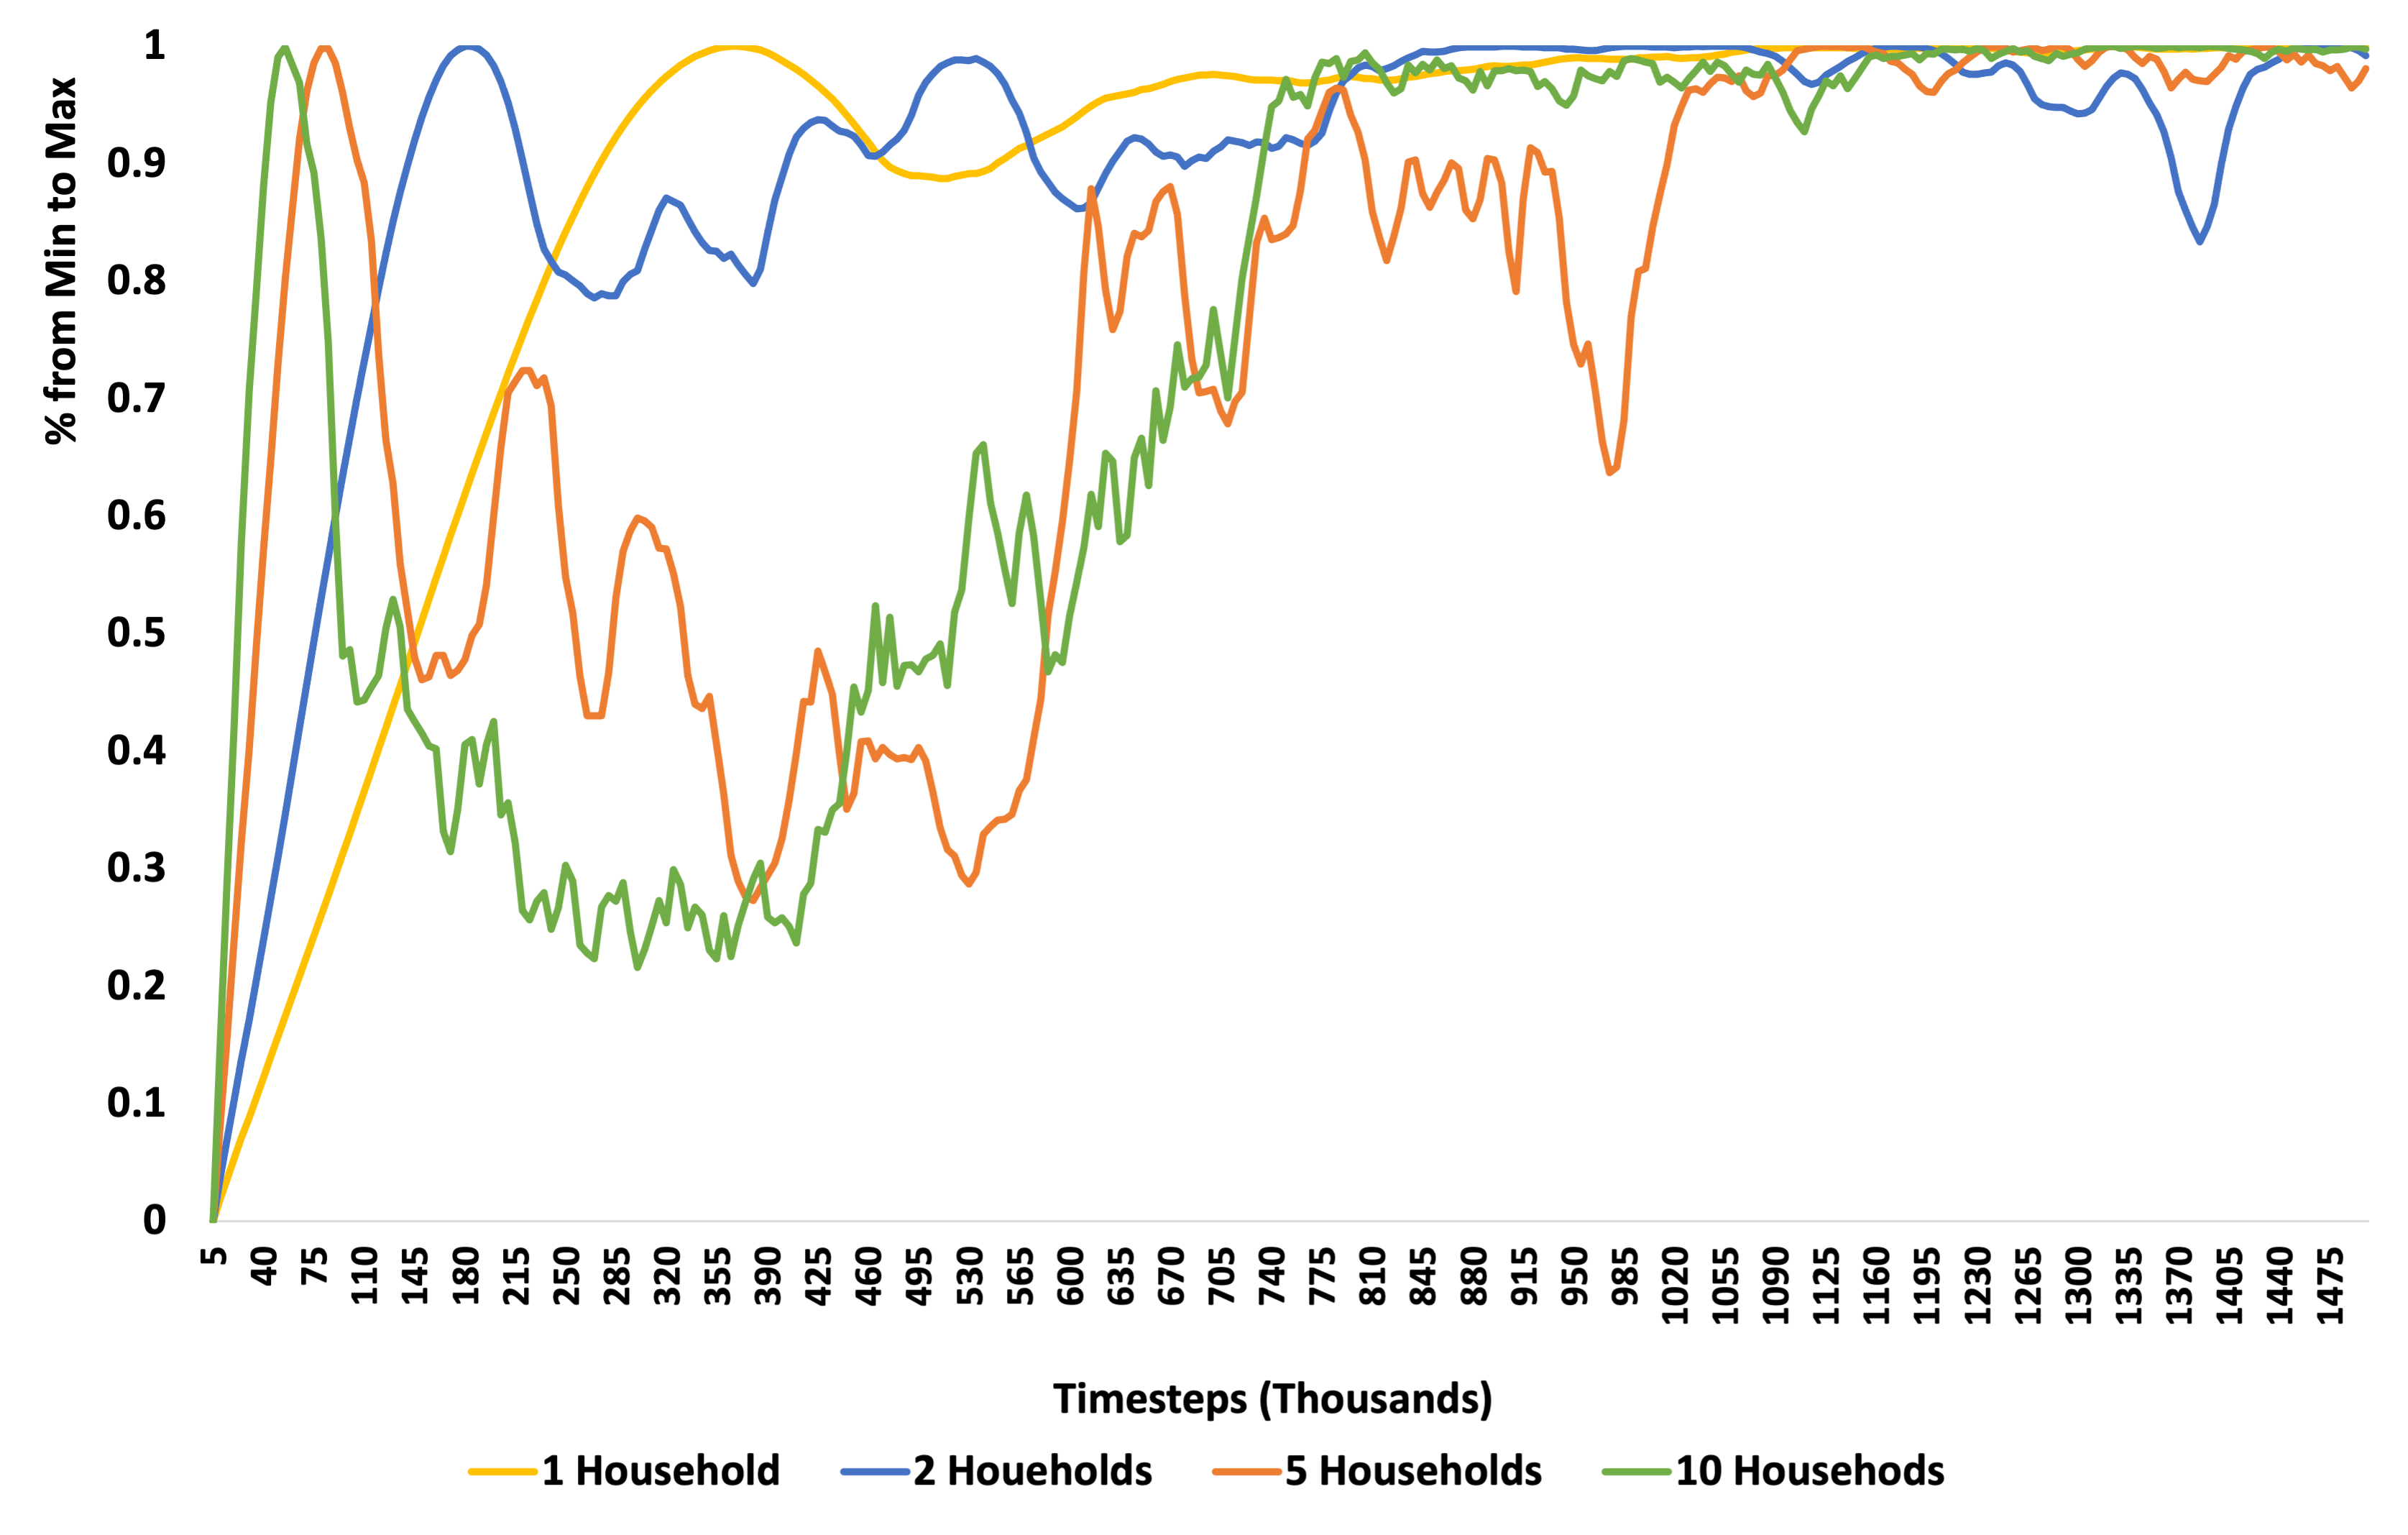
\includegraphics[scale=0.28]{\dir/Learning_graph_planner.png}
\end{figure}
\item The number of transitions needed to reach the peak decreases with amount of households.
\item  Even though the problem is more complex, each transitions convey more information given that we are using a centralized learner with decentralized execution. 

\end{itemize}

\end{frame}

\begin{frame}
\frametitle{Planner, solving for $N^h$ actions instead of only one map.}

\begin{itemize}
	
	\item We now compare scalability in the case when we solve map from the global state to $N^h$ policies.
	
	\begin{figure}
		\centering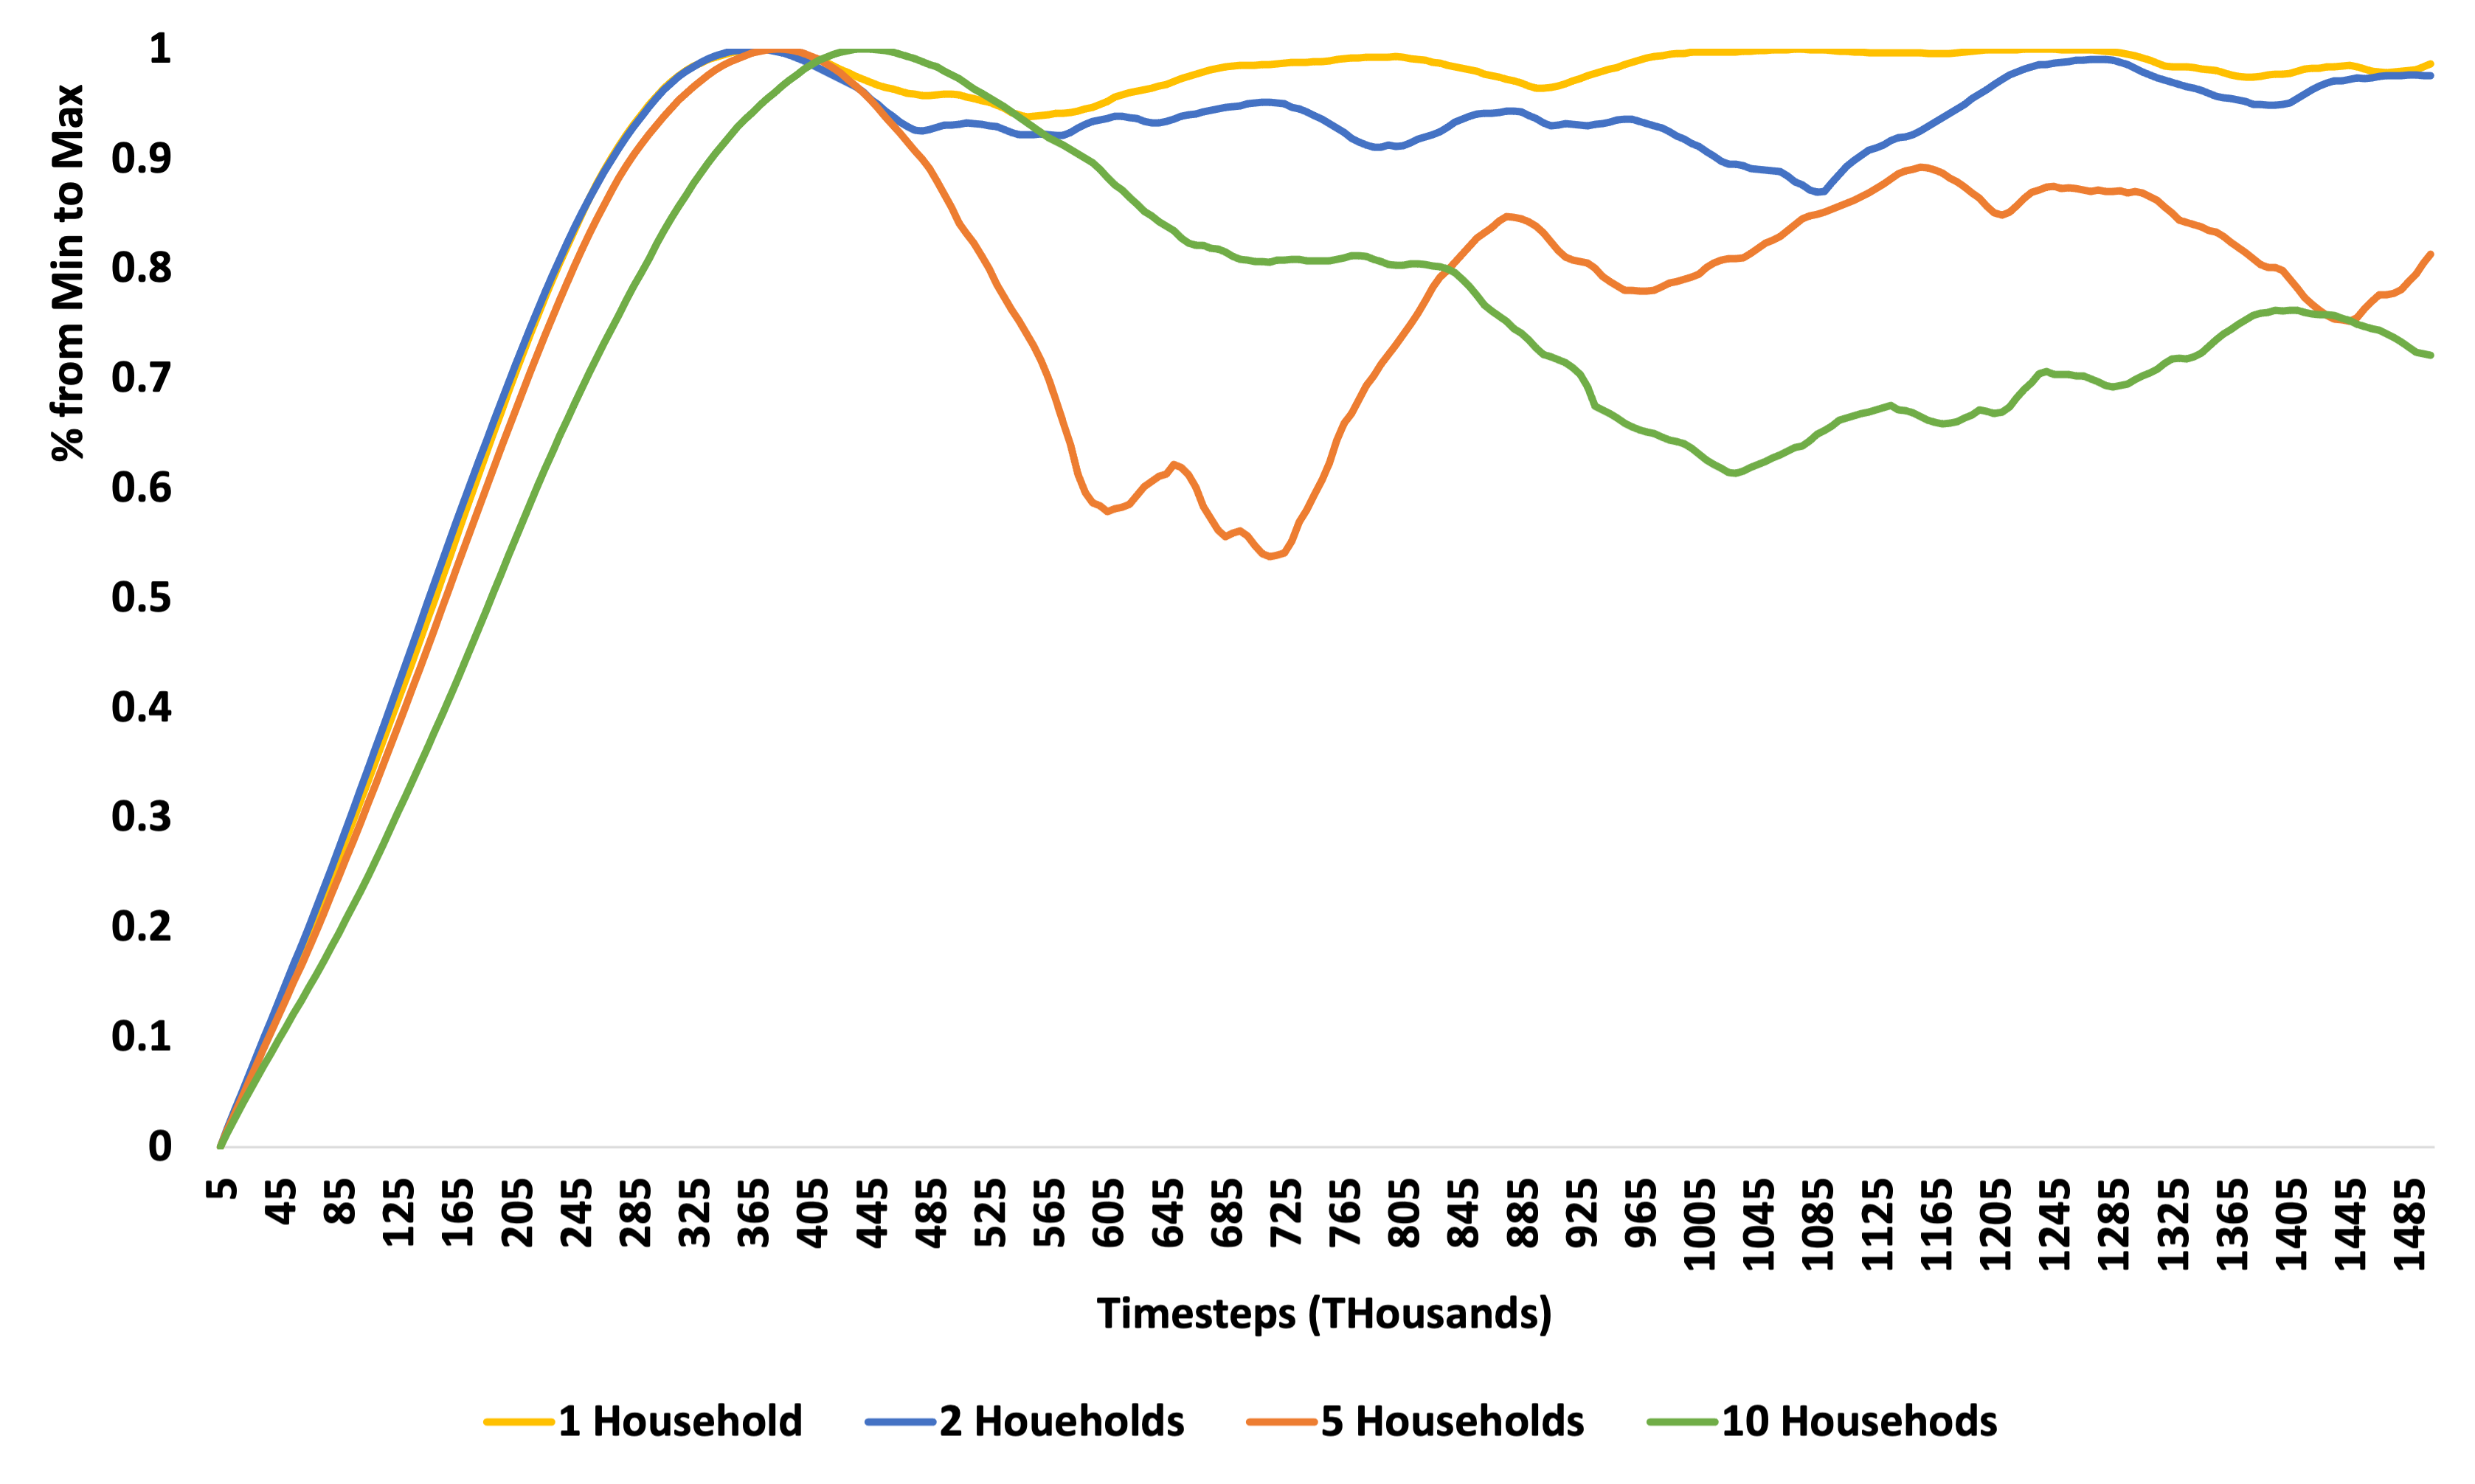
\includegraphics[scale=0.28]{\dir/Learning_graph_planner_sa.png}
	\end{figure}
	\item We still observe scalability, but now the timesteps required to converge increase monotonically.

\end{itemize}

\end{frame}

\begin{frame}
\frametitle{Planner, 1 household (3 state variables)}
	\begin{figure}
	\centering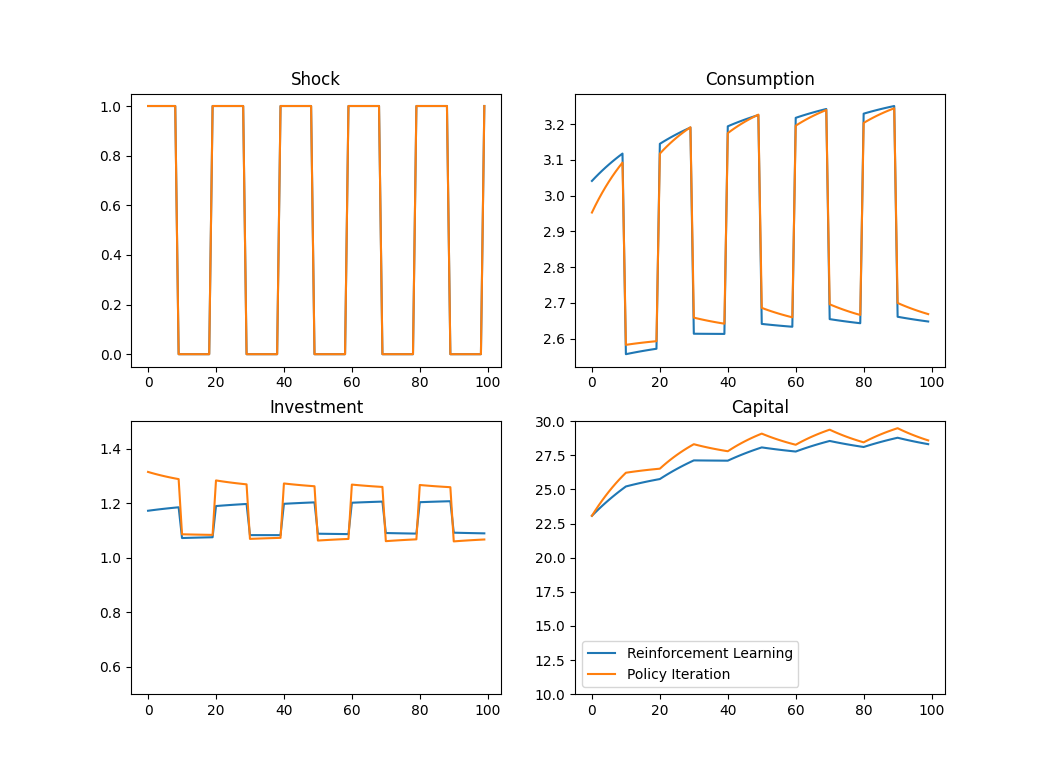
\includegraphics[scale=0.4]{\dir/econ_v_srl_1hh_July29.png}
\end{figure}
\end{frame}

%\begin{frame}
%\frametitle{Planner, 2 households (5 state variables)}
%\begin{figure}
%\centering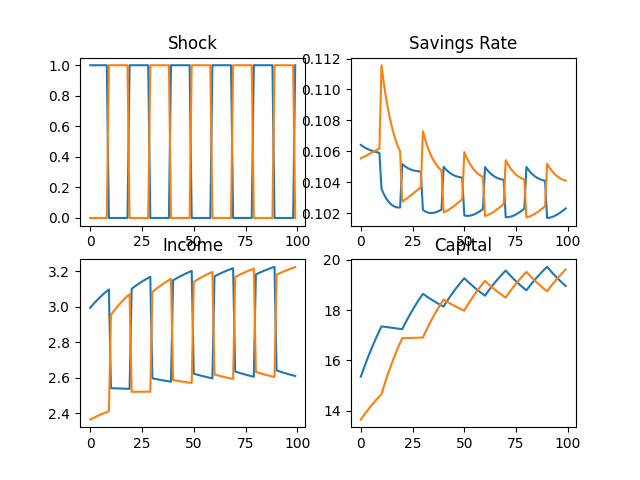
\includegraphics[scale=0.6]{\dir/capital_planner_ma_IR_July22_2hh.png}
%\end{figure}
%\end{frame}

\begin{frame}
\frametitle{Comments on learning}

\begin{itemize}
	\item Learning is fast even in high dimensional problems. Time to reach the peak using only three physical cores: \ms
	\begin{itemize}
		\item 1 HH (3 state variables): 3 minutes 21 second. \ms
		\item 2 HHs (5 state variables): 1 minute 54 seconds. \ms
		\item 5 HHs (11 state variables): 1 min 10 seconds. \ms
		\item 10 HH (21 state variables): 1 min 13 seconds. \ms
	\end{itemize}

	\item For very large problems (e.g., 100 households), the centralized learning approach faces a bottleneck in that the environment needs to pass the whole state space to each household. That could be fixed. \ms
	
	\item In those cases, modeling the problem as finding a mapping from the global state to many different policies (which is slower for lower dimensions), works, but it requires parallelizing over more cores as it takes hours instead of minutes.
	
	

\end{itemize}
\end{frame}









%%% SLIDE 13 %%%


\end{document} 